\chapter{Literature Review}
\label{cha:literaturereview}

%NEED a general intro for chapter

\section{Heating}

The thermal requirements for the extractor to be developed, as outlined in Chapter \ref{cha:introduction}, are very similar in nature to those of a Polymerase Chain reaction (PCR) Thermal Cycling Device, albeit with simplified operations. The requirements of a PCR thermal cycler are driven by the need to cycle the temperature of an array of tubes containing a small volume of sample liquid through temperatures of 55$\degree$C, 72$\degree$C, followed by 92$\degree$C \cite{14405884}. Due to the process involving upwards of 20 cycles between these temperature set points, ramp times for these changes in steady steady state must also be minimised to ensure the total processing time is commercially viable. The thermal requirements of the Gene-Plex Extractor are highly matched, with two exceptions. In this application the temperature of the sample liquid shall be held at a constant 60$\degree$C, as determined by research conducted by AusDiagnostics, as opposed to the multiple temperatures of a PCR cycler. Secondly, the cool down ramp rates for a PCR cycler are of equal importance to it's ramp rates during heating, in order to achieve temperatures lower than the current steady state in adequate times \cite{2563996}\cite{15156909}. In the application of the Gene-Plex Extractor, there is no need to pay attention to cooling ramp rates as the system will only cool at the completion of its operation. Due to the similarities evident between these two applications, a great deal of information may be gathered from PCR cycler design.\\

In order to generate the heat necessary to reach the required sample temperature, some form of thermal pump is required. A Thermoelectric Cooler (TEC), also know as a Peltier, is often used for liquid sample thermal cycling \cite{12436620} among its many other applications. A TEC is a solid state heat pump, controlled by the directional application of electric current across it's two terminals \cite{20160801988967}. The direction of the applied current determines the direction of heat pumping across the module \cite{20160801988967}. TEC's are constructed of pellets of n-type and p-type bismuth telluride semiconductors, connected in an alternating series \cite{6464884}. The connections, made of copper, are bound to a substrate of ceramic alumina. This substrate forms the surface by which the heat generated is transferred. Figure \ref{fig:tec} displays the arrangement of a TEC in a general case application. The TEC has shown through the reviewed literature to be common in PCR thermal cycler applications due to the above mentioned ability to pump heat in either direction, allowing ramping of temperature to be precisely controlled equally in both directions.\\

\begin{figure}[!htb]
	\centering
	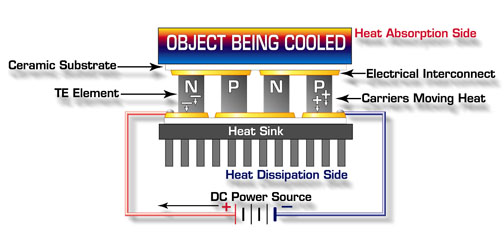
\includegraphics[width = \textwidth]{tec.jpg}
	\caption[Thermoelectric Module Application.]{Thermoelectric module as assembled in a typical application. \cite{Ferrotec}}
	\label{fig:tec}
\end{figure}ˆ 
\FloatBarrier

When used in control applications, a TEC has the advantage of being able to not only add but to also remove heat energy as is required by the controller to achieve the desired response. Despite the TEC's ability to actively remove heat from a component, other active temperature removal methods may also be implemented. A passive approach to heat removal is that employed by a heat sink, or any simple surface area \cite{2006289990179}\cite{20144600208116}. This differs from an active approach, where airflow over the heat sink surface area is controlled via a fan, for example \cite{2006289990179}. Such methods may be substituted for the directional heat pumping capabilities of the TEC, in order to achieve a similar level of temperature control. This leads to simpler possible options for heat pump selection, namely electric resistive heaters. Despite no reviewed literature describing these devices as the main heat source in thermal control for PCR in particular, they have been demonstrated to provide a crucial supporting role by Williams et al. The thermal cycler described in the work of Williams utilizes resistive heat strips to control the temperature of a sealing lid, preventing sample evaporation at the upper operating temperatures of a PCR thermal cycler \cite{7238517}. While the application noted here differs from the intended application within the extractor, where the device will be the primary source of heat, Gene-Plex Extractor, it demonstrates the feasibility of driving component temperature to a steady state value and hence represents a design possibility.\\

\section{Cooling}
In order to be able to control the temperature of the liquid sample as required, a method of evacuating heat must be present. A passive method alone, such as a heat sink in isolation, will not allow the process controller to drive a reduction in heat beyond the limits of conduction to the surrounding air \cite{20144600208116} and as such performance will not be satisfactory. Along with heat dissipation being essential for control, the TEC elements have a maximum temperature differential of which they are capable of generating across their surfaces. This imposes the following constraint on the thermal system:
\begin{equation}
T_{hot} - T_{cold} \leq dT_{max}
\end{equation}
This has been noted as highly significant in PCR cycler design \cite{20160801988967}, where one end of the TEC must be kept at ambient temperature to enable the maximum steady state value of 92$\degree$C to be reached safely. It should be noted that due to the maximum steady state temperature in this application being limited to 60$\degree$C and assuming a reasonable TEC differential limit, $dT_{max}$, this constraint is not critical. However, a TEC becomes less efficient as it's temperature differential is increased \cite{20070113880}. As such, a method of heat evacuation must be present.\\
%FOR last sentence, it is more correct to state that it is desirable to maintain a heatsink temperature at room temp to minimise differential

%NOTE: for the above explanation, include a graph of peltier temperature differential vs power transfered, as http://www.heatsink-guide.com/peltier.htm. This is in widomski.

\section{Controllability}
\label{lit_controlability}
In order to create a thermal system which is controllable within the context of stability and speed of response, attention must be paid to the thermodynamics of the device. Due to manufacturing constraints and standards, the tube which contains the sample itself is not optimal. A wall thickness of 1mm results in poor heat transfer characteristics from the heated block to the sample \cite{1704922}. Another source of poor dynamics is any regions of mechanical connection between the heated block and external components \cite{7238517}. Recommendations from the reviewed literature included the use of gasket material to limit thermal material between any surface contacts (Williams et al specifically recommends the use of ethylene propylene), along with the use of a groove extending through the majority of the thickness and hence limiting heat transfer to the mechanical connections \cite{20130415930883}\cite{20070113880}. Mechanical connections are however only one cause of significant thermal gradient within the device. Care must be taken to reduce the severity and frequency of the occurrence of these gradients to maintain stability and performance in temperature response. After heat pumping has ceased, a temperature gradient will persist for a period of time that is proportional to the square of the distance between the hot and cold locations \cite{7238517}. This has important implications for the number of sample tubes that may be heated within a single block. If the size of the sample array to be heated is too large, difficulty will be encountered achieving a uniform and stable steady state temperature \cite{7238517}. Widomski et al note that despite efforts to reduce heat loss and hence gradients around the system boundaries via methods such as insulation, the region of location of the heat source will continue to maintain a higher temperature. To counter this, it is suggested to use a rod of material with lower thermal conductivity (such as stainless steel within an aluminium block) to reduce the heat retained in this volume \cite{20070113880}.\\
%INLCUDE 	equation for time of gradient

A number of measures may also be taken directly related to the heated block itself to ensure optimal thermal response. The concepts of static local balance and static local symmetry may be applied to obtain desirable heat transfer within the medium \cite{7238517}. A state of static local balance refers to a state of constant temperature where all heat sinks are equalled by heat sources in a local area \cite{7238517}. This essentially describes a state of thermal equilibrium, where the following condition is satisfied:
\begin{equation}
Q_{in} = Q_{out}
\end{equation}
To ensure this balance is obtained, a device design should not incorporate overly effective heat sinks, without a proportional increase in the heat source capacity, and visa versa. The condition of static local symmetry requires that for a constant temperature and within a local region, the center of mass of the heat source is coincident to the center of mass of the heat sink \cite{7238517}. Satisfying this condition will ensure that a constant, steady state temperature is achievable, without the presence of a permanent temperature gradient between the two centers of mass. The selection of heated block material along with manufacturing methods may also act to improve transfer properties. Aluminium 6061 is recommended due to its purity \cite{7238517}, which aids in even heat transfer \cite{OLAFSSON1997}. It is further recommended that the heated block be manufactured via machining, due to the homogeneous structure that results. This is beneficial in reducing any temperature gradients that may occur within the heated element due to mechanically or otherwise joined components or impurities or inconstancies that exist as a result of other manufacturing methods such as casting.

\section{Temperature Sensors}
The literature reviewed has presented various differing selections of temperature sensing technologies, the most prominent of which have been thermocouples and thermistors. Despite the overlapping application, the specifications of the two technologies are significantly different. The thermocouple has a large temperature range, with measurements capable of ranging from -270$\degree$C to 1800$\degree$C compared to the limited range of thermistors of usually around -90$\degree$C to 130$\degree$C \cite{11303490}\cite{15156909}\cite{10650397}. The thermocouple and thermistor possess similar response rates along with similar accuracy, however due to the wider resistance range available, thermistors are able to achieve a high measurement resolution \cite{11303490}\cite{15156909}\cite{10650397}. The two significant differences between the technologies are power supply requirements and linearity. Due to the welding of differing metal conductors at the measuring point, the thermoelectric effect results in a temperature dependant voltage being generated across the thermocouple terminals \cite{11303490}\cite{10650397}\cite{15156909}. While this means the sensor does not require a power supply, it can introduce complications requiring a reference/compensating wire. Furthermore, changes to the conductor materials such as corrosion require that the sensor be calibrated on a regular basis, often as frequently as 3 months \cite{11303490}\cite{15156909}\cite{10650397}. Thermistors use semi-conductive material that changes resistance with temperature. As such, measuring the temperature requires a current be passed through the device \cite{11303490}\cite{15156909}. While the output voltage of thermocouples changes linearly with temperature, this is not true of thermistors. Hence, the output signal requires linearisation before it may be of use \cite{15156909}. In commercial applications, thermistor technology is often also preferred due to its cost effectiveness \cite{10650397}. While Resistive Thermal Detectors (RTD's) and Integrated Temperature Sensors appeared in a number of reviewed sources, they are not considered in depth due to the high level of signal conditioning required \cite{10650397}\cite{11303490} and the lack of observed uses in relevant thermal control applications.

\section{Temperature Sensing}
To utilize the thermal system to control the liquid sample temperature accurately, a method of obtaining a feedback signal is required. Complications exist however due to the constraint that the sample temperature itself cannot be directly measured. Due to the thermal transfer characteristics discussed above, the placement of the sensing device is critical to the stability of the controlled substance \cite{20130415930883}. Vilchiz et al studied the issues of sensor hardware placement and provide numerous recommendations to increase baseline stability. Using experimental methods, it was verified that the following one-dimensional heat equation holds:
\begin{equation}\label{time lag}
s=\frac{L}{a}
\end{equation}
Where $s$ is the time taken for energy to flow from location A to location B, $L$ is the distance between the two locations, and $a$ is the thermal diffusivity of the material. This is relevant as it allows the time lag between a controlled heating action at the heat source to the arrival of the generated heat at the location of interest to be determined. The experiment conducted tested two temperature sensing cases. One sensor was placed within the center of mass of the heated block, while the other was located as close as was possible to the heat source. The results obtained found that ``there is a general advantage of control via sensing close to the heater, whether by temperature measurement, or by heat-flow control sensing.'' \cite{20130415930883}. Equation \ref{time lag} is accountable for this result. When the sensor is placed at a greater distance to the heat source, the control effort is determined using a measurement that is not yet equalised due to the more severe temperature gradient. This error in feedback signal is reduced by the recommended placement strategy, such that ``the reduction in the magnitude of the heater-induced oscillations achieved by this control strategy is at least one order of magnitude better than that of the temperature control at the core'' \cite{20130415930883}.\\
%FOR above quote, either show figure of this repsonse (ideal) or make note that response oscillated

A number of aspects of the experiments and findings the work of Wilchiz et al should however be considered. The sensing device used to make the presented conclusions were thermocouples, one of many sensing devices available. Despite the variances in accuracy and stability of measurements that are expected between differing sensing technologies, the results can be assumed independent of any associated error. Any error as a result of sensor output stability is of an insignificant order to magnitude of time when compared to the 1.07 min thermal lag situation generated by the experiment. Furthermore, one would expect a sensor technology of differing accuracy to produce a controlled output different to the desired reference input. This error is however not influential to the results given, which are concerned exclusively with the stability of the controlled response. The focus of the experiment was the application of thermocouple technology in Tian-Calvet microcalorimeter devices. This does not detract from the relevance of the reviewed work for a number of reasons. The motivation for the study was to improve baseline stability in temperature control, via the application of improved temperature measurement strategies; a general outcome that is relevant to the work of this thesis. Further to this, the scale of the experiment conducted closely resembles the device to be developed, with the distance between sensor locations set equal to 3.5cm. Therefore, despite the differing applications of the work conducted, the recommendations and strategies found may be concluded as directly applicable.

\section{Controller Design}
With the necessary hardware in place and optimally set up, as has been discussed above, controller design and theory may be considered. The large majority of the reviewed literature, along with the instruments currently employed by AusDiagnostics, recommend or employ the Proportional Integral Derivative (PID) controller. As summarised by Vilchiz et al, ``Although other types of controllers are also feasible, e.g., those based on fuzzy logic or artificial neural networks, the simplicity, good response, and low cost of PID-based control loops have motivated their popularity in industrial applications'' \cite{20130415930883}\cite{20160801988967}. Despite the common application of the PID controller in thermal control applications, if a TEC is the selected source of heat, complications are presented. Due to the non-linearity of the device, PID coefficient selection involves the process of trial and error \cite{20160801988967}. The strategies for PID design given were however applied to the thermal cycling requirements of PCR. This requires that 3 separate temperature controllers be implemented for each of the temperature set points, to ensure the required performance is met equally at each \cite{20160801988967}. While the characteristics of the PID controller are not effected by this difference, it does significantly increase the complications of coefficient selection in comparision to the application in the Gene-Plex Extractor. Further to the controller to be implemented itself, a number of sources give recommendations regarding relevant hardware. Cellatoglu et al investigated the dynamic performance of a process control system, with a focus on temperature controllers. The findings reveal that the word length of the ADC utilised is an important factor in reducing output error. A case study was conducted to assess the impact of increased word length on error, with results suggesting that 8 bits is the optimal value \cite{12096602}. It was further found that an increase in word length beyond this point yields no reduction in error. The analysis conducted was however completed as a simulation, with no experimental verification evident. The electronic hardware implemented in other sources, such as the work of Shirafkan et al, differs from this recommendation. While  not providing evidence to suggest the 8-bit recommendation is problematic, the successfully implemented controller utilized a 24-bit ADC.\\

%NOTE: fIGURE FOR ADC WORD LENGTH?
\section{Magnetic Separation}
To ensure the target DNA is extracted as required, the device must include a robust means of capturing the magnetic beads. Despite offering an alternative means of magnetic bead manipulation, electromagnets are not investigated for application in the thesis due to a high level of complexity that is not required for this static, constant force implementation. Therefore, the review of literature focuses on permanent magnets. While there are numerous compositions of magnets available, the rare earth variety and in particular the Neodymium composition (ND-Fe-B) are most suitable. Neodymium magnets offer the strongest solution, with an energy product of up to 56 MGOe \cite{2006189852255}. Good mechanical characteristics and energy to size ratio make them suitable for fastening within a manufactured product, without undue difficulty. Importantly, given the requirement to capture beads within the heated block element, Neodymium magnets are stable in temperatures near ambient. Progressive loss of magnetism occurs at temperatures greater than 80$\degree$C \cite{2006189852255}, providing a 20$\degree$C margin of safety between the operating temperature of 60$\degree$C. This composition also holds a very high coercive force \cite{2006189852255}, allowing it to resist demagnetisation in the presence of external magnetic fields that will be present within the Gene-Plex Extractor, as a result of other hardware. Despite the specification of the superparamagnetic silica beads being a constraint determined by completed research at AusDiagnostics, a number of characteristics should be noted in order to obtain reliable bead capture capabilities. Shevkoplyas et al describes the force acting an a superparamagnetic bead due to an applied force. The context of this paper is the motion prescribed by the beads within a microfuidic chamber, however the general characteristics of the interaction between the beads and magnetic field are applicable to the capture required here. In order to saturate a suspension of superparamagnetic beads, an external magnetic field greater than 0.5T must be applied \cite{9774403}. Saturation is the state where all beads magnetic poles are aligned. In a state of saturation, the magnetic beads behave simply as permanent magnets \cite{9774403}\cite{8667402}. In order to ensure the complete separation of the magnetic bead dispersion within the sample liquid, this condition must be achieved.\\
% NEED to elaborate on magnetic capture. Also give equations and figures to show.

The literature reviewed has allowed a number of critical elements of thermal control and magnetic separation, being the main requirements of the extraction system, to be recognised and evaluated within the context of this thesis. The similarity between the processes demanded by the extraction technique and the works discussed allow the information gathered to be applied directly to the benefit of the developed instrument. Those works which were an exception to this allowed general strategies and design characteristics to be collected, which may be applied with consideration in future development.

%NOTE: NEED TO INCLUDE SOME HALBACH ARRAY